\section{Ejercicio 2}
\noindent
En la presente sección se planea diseñar e implementar una maquina de estados que analice la secuencia de bits en forma sincrónica de tal forma que encienda una salida cuando reconozca la secuencia de numeros 1-1-0-1 en su entrada.\\
Para ello se utilizará una Máquina de Mealy, de esta manera, se muestra a continuación el diagrama de estados correspondientea a dicha situación en la figura \ref{ej2_estados}
%
\begin{figure}[H]
    \centering
    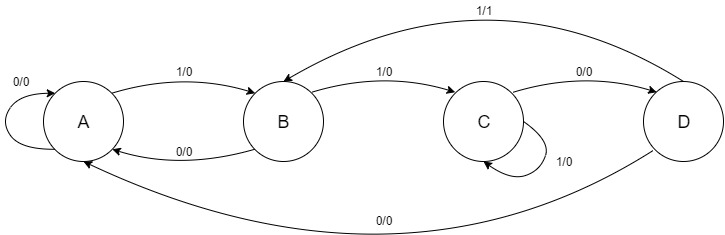
\includegraphics[width=0.8\textwidth]{figs/Ej2/diag_estados.jpg} % first figure itself
    \caption{Diagrama de estados del circuito a realizar.}
    \label{ej2_estados}
\end{figure}
%
De esta manera, la tabla de transisciones queda de la forma de la tabla \ref{ej2_tabla1}.
%
\begin{table}[H]
\caption{Tabla de Estados.}
\label{ej2_tabla1}
\centering
\begin{tabular}{|c|c|c|c|c|c|}
\hline
\multicolumn{2}{|c|}{Estado Actual}             & \multicolumn{2}{c|}{Estado Siguiente} & \multicolumn{2}{c|}{Salida}                 \\ \hline
\multirow{2}{*}{Nombre} & \multirow{2}{*}{y2y1} & W=0               & W=1               & \multirow{2}{*}{W=0} & \multirow{2}{*}{W=1} \\ \cline{3-4}
                        &                       & Y2Y1              & Y2Y1              &                      &                      \\ \hline
A                       & 00                    & 00                & 01                & 0                    & 0                    \\ \hline
B                       & 01                    & 00                & 11                & 0                    & 0                    \\ \hline
C                       & 11                    & 10                & 11                & 0                    & 0                    \\ \hline
D                       & 10                    & 00                & 01                & 0                    & 1                    \\ \hline
\end{tabular}
\end{table}
%
 \noindent
 Así, los mapas de Karnaugh a realizar se pueden ver a continuación, donde A,B,C son y2, y1, W respectivamente.\\
Y1:
%
\begin{center}
    \begin{Karnaughvuit}
       \minterms{4,5,6,7}
        \maxterms{0,1,2,3}
       \implicant{4}{6}{red}
    \end{Karnaughvuit}
\end{center}
%
Y2:
%
\begin{center}
    \begin{Karnaughvuit}
       \minterms{5,7,3}
        \maxterms{0,1,2,4,6}
       \implicant{5}{7}{blue}
       \implicant{3}{7}{green}
    \end{Karnaughvuit}
\end{center}
%
Z:
%
\begin{center}
    \begin{Karnaughvuit}
       \minterms{6}
        \maxterms{0,1,2,3,4,5,7}
        \implicantsol{6}{purple}
    \end{Karnaughvuit}
\end{center}
%
\noindent
Así de esta forma las ecuaciones que se encuentran a partir de los mapas de kernaugh mostrados se pueden ver en las ecuaciones \ref{ej2_eq}.
%
\begin{equation}
\begin{split}
    Y1&=W\\
    Y2&=y1\cdot W+y1\cdot y2 = y1(W+y2)\\
    Z&=y2\cdot \overline{y1}\cdot W
\label{ej2_eq}
\end{split}
\end{equation}
%
Así se puede llegar al circuito de la figura \ref{ej2_circuito.}.
%
\begin{figure}[H]
    \centering
    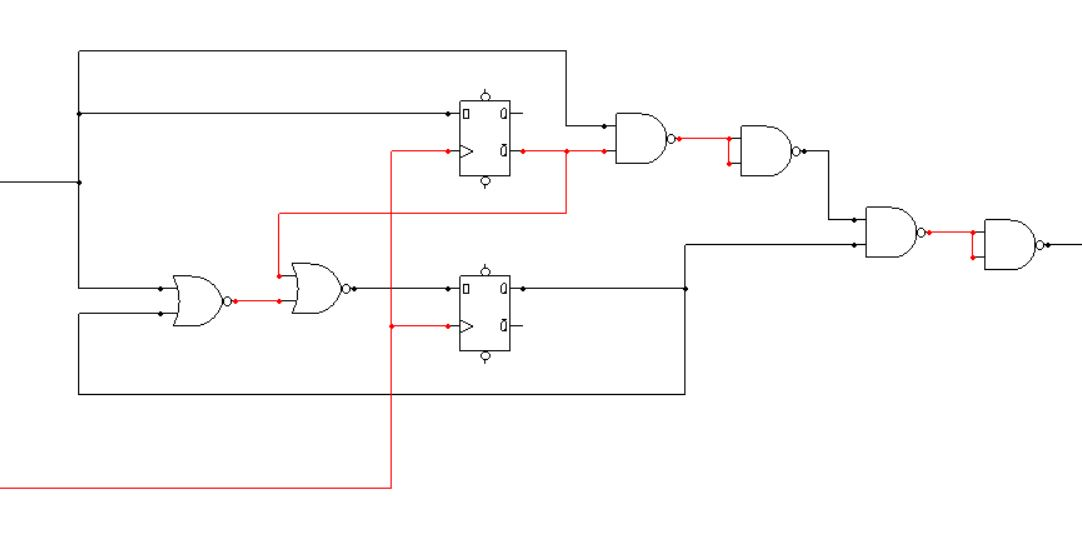
\includegraphics[width=0.8\textwidth]{figs/Ej2/circuit_ej2.JPG} % first figure itself
    \caption{Imagen esquemática del circuito realizado.}
    \label{ej2_circuito.}
\end{figure}
%
Luego se pasó a medir el circuito, para ello se comprobó que todas las secuencias lógicas funcionen de forma correcta al ser testeadas las mismas.\\
De esta manera se procede a mostrar los resultados de las mediciones tomadas para el circuito en cuestión.\\
Para comenzar se muestran en la figura \ref{ej2_resultados1} cómo la salida se activa al detectar el circuito la secuencia de numeros deseado.\\
En verse se puede ver el clock, en violeta la entrada del sistema y en amarillo la salida del mismo.
%
\begin{figure}[H]
    \centering
    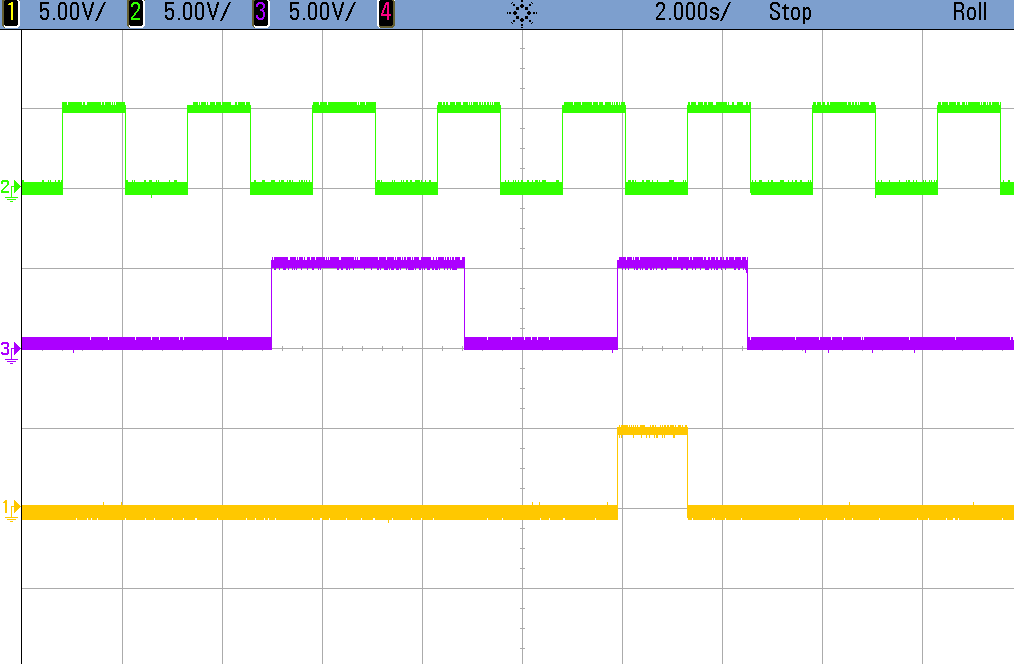
\includegraphics[width=0.6\textwidth]{figs/Ej2/scope_14.png} % first figure itself
    \caption{Mediciones tomadas del circuito, donde se ve como la salida se activa al entrar la secuencia buscada, 1-1-0-1.}
    \label{ej2_resultados1}
\end{figure}
%
Luego en la imagen \ref{ej2_resultados2} se puede ver como el sistema responde de acuerdo a lo esperado al entrar con 1-1-0-1-1-0-1.

%
\begin{figure}[H]
    \centering
    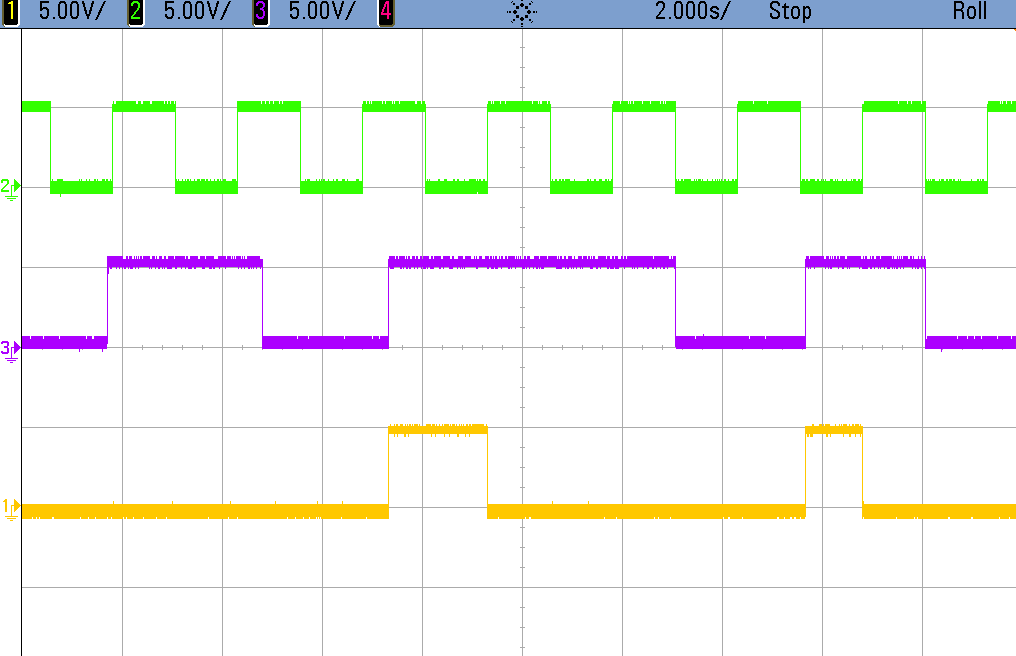
\includegraphics[width=0.6\textwidth]{figs/Ej2/scope_155.png} % first figure itself
    \caption{Mediciones tomadas del circuito, donde se ve como la salida se activa 2 veces con la entrada 1-1-0-1-1-0-1}
    \label{ej2_resultados2}
\end{figure}
%
De esta manera podemos concluir que el circuito funciona de acuerdo a lo esperado, obteniéndose los resultados deseados con el mismo.